\documentclass[pdflatex,sn-mathphys-num]{sn-jnl}

\usepackage{graphicx}
\usepackage{amsmath,amssymb,amsfonts}
\usepackage{booktabs}
\usepackage{xcolor}
\usepackage{url}
\usepackage{hyperref}

\begin{document}

\title[HeatTrace Dataset and Benchmark]{HeatTrace: A Historical Heatwave Dataset and Evaluation Benchmark for Sustainable Cloud Scheduling}

\author*[1]{\fnm{[AUTHOR NAME(S)} \sur{--- CONFIRM]}}\email{[CORRESPONDING AUTHOR EMAIL --- CONFIRM]}
\affil*[1]{\orgdiv{[DEPARTMENT --- CONFIRM]}, \orgname{[INSTITUTION --- CONFIRM]}, \orgaddress{\city{[CITY --- CONFIRM]}, \state{[STATE --- CONFIRM]}, \country{[COUNTRY --- CONFIRM]}}}

\abstract{Sustainable cloud schedulers are commonly evaluated on ordinary historical periods, although sustained heat can change modeled cooling overhead and usable IT capacity. HeatTrace is a historical heatwave dataset-construction pipeline and evaluation benchmark that aligns NOAA hourly weather observations, CAISO wholesale electricity prices, and EIA grid-system records; detects events from weather alone; and materializes complete-event, matched-control, and event-blind windows with machine-readable provenance. The original single-station California catalogue contains four SFO events over June--September 2022--2025, one development triplet and three confirmatory triplets, each represented by 120 hourly rows. A five-station extension covering 2022--2026 contains 25 station events grouped into 15 regional episodes: 12 events are eligible, nine 2022 events are excluded, and four 2026 events are provisional. Public measurements remain distinguishable from HeatTrace-derived labels and synthetic scheduling inputs. Benchmark utility is demonstrated with a frozen 756-cell scheduling evaluation. Two of three confirmatory events showed a 0.5$\times$ lower seed-averaged tested static boundary; two showed 24/36 nonzero equal-service policy separations where selected ordinary windows showed 0/36. The third event was null, one matched control also showed 24/36, and no strict ranking reversal occurred. A same-environment rerun reproduced all 756 cells and 44 audited scientific columns. The multi-station catalogue is useful dataset development, but forecast transfer, service attrition, and overlapping ordinary windows prevent validation of its forecast-aware scheduling conclusions.}

\keywords{Historical heatwave dataset, sustainable cloud scheduling, evaluation benchmark, data provenance, power usage effectiveness, reproducibility}

\maketitle

\section{Introduction}\label{sec:intro}

Delay-tolerant computation can be shifted toward lower-price or lower-carbon periods, but the apparent benefit depends on workload constraints, electricity signals, and facility overheads \cite{radovanovic2023carbon,wiesner2021let,hanafy2023carbonscaler}. Ambient heat can raise modeled cooling demand and reduce usable IT power under a facility cap. An evaluation restricted to benign or arbitrary periods may therefore omit conditions in which feasibility and policy differences emerge. Yet an extreme-event benchmark can also mislead if it selects events using outcomes, treats simulation cells as independent weather observations, compares unequal completed work, or interprets production-average carbon as avoided emissions.

HeatTrace addresses the data and evaluation problem rather than proposing a new scheduler. Its primary contribution is a reproducible pipeline for acquiring and harmonizing historical weather and electricity-system data, identifying complete heatwaves, constructing matched and event-blind scenarios, recording source and quality metadata, and freezing machine-readable benchmark artifacts. The source observations were collected by NOAA, CAISO, and EIA; HeatTrace contributes derived alignments, event labels, catalogues, windows, manifests, and evaluation tables. Synthetic workloads and thermal responses are a third layer used only to demonstrate benchmark utility.

The secondary contribution is an event-conditioned scheduling case study that retains null results and enforces equal service. The tertiary contribution audits source coverage, identifiers, hashes, frozen specifications, same-environment reproduction, and an exploratory multi-station extension whose experimental conclusions remain unvalidated.

The study is deliberately bounded. The original benchmark has three independent confirmatory triplets ($N=3$), not 756 independent events. CAISO prices are wholesale hub signals, EIA carbon is a balancing-authority production average, and the facility and workloads are modeled sensitivities rather than telemetry. No global discriminability, causal forecasting benefit, or physical outage effect is claimed.

\section{Related Work and Dataset Research Gap}\label{sec:related}

Temperature-aware placement and environmentally aware scheduling are established areas. Thermal observations have guided workload placement and cooling efficiency \cite{moore2005making}; GreenSlot aligned deadline-constrained work with renewable availability \cite{goiri2011greenslot}; and Liu et al. coordinated cooling, outdoor temperature, renewables, and workload management \cite{liu2012renewable}. Carbon-aware systems have examined fleet-scale temporal shifting \cite{radovanovic2023carbon}, deadline and regional trade-offs \cite{wiesner2021let}, workload elasticity \cite{hanafy2023carbonscaler}, operational and embodied carbon \cite{acun2023carbon}, and limits on temporal and spatial shifting \cite{sukprasert2024limitations}. These studies motivate environmental awareness but do not by themselves specify an outcome-blind, complete-heatwave dataset protocol.

Recent benchmarks broaden data and evaluation scope. DCcluster-Opt combines weather, price, carbon, network, and data-center models across regions \cite{guillenperez2025dccluster}; WeatherBench~2 standardizes global weather-forecast data and evaluation \cite{rasp2024weatherbench}; and ExtremeWeather provides gridded event-detection data \cite{racah2017extremeweather}. These resources answer different questions: the first supports multi-objective data-center optimization, the second compares weather forecasts, and the third supports detection in gridded climate fields. HeatTrace instead contributes a derived catalogue of complete station-observed heatwaves, outcome-blind controls and ordinary windows, explicit quality and eligibility flags, source-to-artifact manifests, and a scheduling evaluation protocol. Its California scope is narrower, and neither its station series nor its modeled facility replaces a global or physics-informed benchmark.

Ruparel studies geo-distributed scheduling with DRO/CVaR, Wasserstein ambiguity sets, decomposition, batteries, and renewables \cite{ruparel2026carbon}. HeatTrace shares the motivation of forecast-aware sustainability but uses greedy/repair policies and a heuristic temperature margin. Its research gap is dataset and benchmark validity under authentic multi-day heat: weather-only selection, complete-event windows, outcome-independent comparators, like-for-like service, and traceable negative results.

\section{HeatTrace Dataset: Sources, Design, and Construction}\label{sec:data}

Figure~\ref{fig:pipeline} separates the three evidence layers. External organizations provide measurements; HeatTrace creates aligned records, labels, windows, and provenance; benchmark simulations add synthetic workloads, modeled thermal capacity, policy outputs, and evaluation metrics. Scheduling results cannot affect event or window eligibility.

\begin{figure*}[t]
\centering
\setlength{\fboxsep}{7pt}
\fcolorbox{blue!55!black}{blue!5}{\parbox[c][1.75cm][c]{0.235\textwidth}{\centering\textbf{External observations}\par\smallskip\small NOAA GHCNh\par CAISO/EIA grid signals}}
\hspace{0.01\textwidth}$\boldsymbol{\longrightarrow}$\hspace{0.01\textwidth}
\fcolorbox{green!45!black}{green!6}{\parbox[c][1.75cm][c]{0.235\textwidth}{\centering\textbf{HeatTrace records}\par\smallskip\small alignment and QC\par events, scenarios, manifests}}
\hspace{0.01\textwidth}$\boldsymbol{\longrightarrow}$\hspace{0.01\textwidth}
\fcolorbox{orange!55!black}{orange!8}{\parbox[c][1.75cm][c]{0.235\textwidth}{\centering\textbf{Benchmark evaluation}\par\smallskip\small workload/PUE\par policy/service metrics}}
\caption{HeatTrace data lifecycle. Public source measurements are preserved separately from newly derived dataset artifacts and from synthetic benchmark inputs. Event selection and scenario construction precede scheduling evaluation.}
\label{fig:pipeline}
\end{figure*}

\subsection{Source measurements and spatial mappings}

The original benchmark uses NOAA Global Historical Climatology Network hourly (GHCNh) observations at San Francisco International Airport (SFO, \texttt{USW00023234}) \cite{noaaGhcnh}. Weather supplies local dry-bulb temperature for event detection and thermal input. Day-ahead locational marginal price comes from the CAISO OASIS NP15 hub \cite{caisoPrices}; EIA-930 CISO records provide demand, net generation, estimated emissions, and production-based carbon-intensity context \cite{eia930}. Stored timestamps are UTC interval starts, while weather-day operations use \texttt{America/Los\_Angeles}. EIA publishes hour-ending values; HeatTrace shifts them to interval starts, converts the workbooks' generated-intensity field from lb/kWh to g/kWh, and independently checks its emissions/positive-generation reconciliation. It does not estimate marginal or avoided emissions.

The extension adds Sacramento (SAC, \texttt{USW00023232}), Fresno (FAT, \texttt{USW00093193}), Redding (RDD, \texttt{USW00024257}), and Los Angeles (LAX, \texttt{USW00023174}), spanning coastal and inland regimes. SFO, SAC, and RDD map to NP15, FAT to ZP26, and LAX to SP15. All share the CISO production-average carbon proxy, precluding station-local carbon inference.

\begin{table*}[t]
\caption{Data layers, study coverage, use, and interpretation limits.}
\label{tab:sources}
\small
\begin{tabular}{@{}p{0.15\textwidth}p{0.20\textwidth}p{0.23\textwidth}p{0.32\textwidth}@{}}
\toprule
\textbf{Layer} & \textbf{Coverage} & \textbf{Use} & \textbf{Limit} \\
\midrule
NOAA GHCNh & Hourly warm-season records; SFO 2022--2025 primary, five stations 2022--2026 extension & Temperature QC, daily maxima, thresholds, event and phase labels & Airport stations are environmental proxies, not facility telemetry; 2026 is provisional \\
CAISO OASIS & Day-ahead hourly NP15, ZP26, or SP15 hub LMP & Cost signal and regional market context & Wholesale hub price, not a retail tariff; historical API availability varies \\
EIA-930 CISO & Hourly demand, generation, emissions, intensity & Grid context and carbon-first objective & Production average, not marginal or avoided emissions; issue flags retained \\
HeatTrace derived & Alignments, catalogues, windows, manifests, result tables & Reusable events, scenarios, QC, and evaluation records & Public derived artifacts are available; the full local hourly extension and provider inputs are excluded \\
Synthetic inputs & Seeded jobs, temperature forecasts, PUE/capacity curves & Scheduling benchmark validation & Not measured workload or facility response \\
\bottomrule
\end{tabular}
\end{table*}

\subsection{Alignment, quality control, and provenance}

Parsers retain provider IDs, query scope, retrieval and processing times, file sizes, SHA-256 digests, coverage counts, and issue status. Weather processing applies NOAA quality codes, resolves duplicates deterministically, converts units, and forms local-day maxima from half-open UTC intervals. Missing weather breaks a qualifying run; no values are imputed. Price, carbon, demand, workload, and scheduling outcomes cannot affect event eligibility. Aligned records retain signals, observation counts, missingness, conflicts, issue flags, mapped price hub, and generated and consumed EIA intensity fields.

\section{Heatwave Event Catalogue and Benchmark Scenarios}\label{sec:catalogue}

\subsection{Original single-station catalogue}

The SFO detector screens 485 valid June--September days in 2022--2025. A heatwave is at least three consecutive local days whose daily maximum strictly exceeds the warm-season empirical $P_{90}$ threshold of $25.60\,^{\circ}\mathrm{C}$. Four events satisfy the rule: June~20, September~4, and September~22 of 2022, and July~2 of 2024.

The primary evaluation windows are fixed at 120 hours and must contain the complete detected event. For an event shorter than 120 hours, unused time is divided symmetrically before and after the event; a 72-hour event receives 24 hours on each side. A 120-hour event receives no padding. Events longer than 120 hours would be ineligible rather than truncated. This is distinct from the variable onset-to-recovery windows retained in the multi-station catalogue.

The July 2024 event forms a development triplet and is excluded from confirmation. The confirmatory triplets pair the three 2022 events with June 2024 controls and equal-duration event-blind warm-season windows. This cross-year matching is an explicit limitation. Controls are selected without scheduling outcomes; event-blind windows are sampled after excluding heatwaves, buffers, matched controls, and incomplete canonical signals. Figure~\ref{fig:signals} illustrates the development event/control pair but is not confirmatory evidence.

\begin{figure*}[t]
\centering
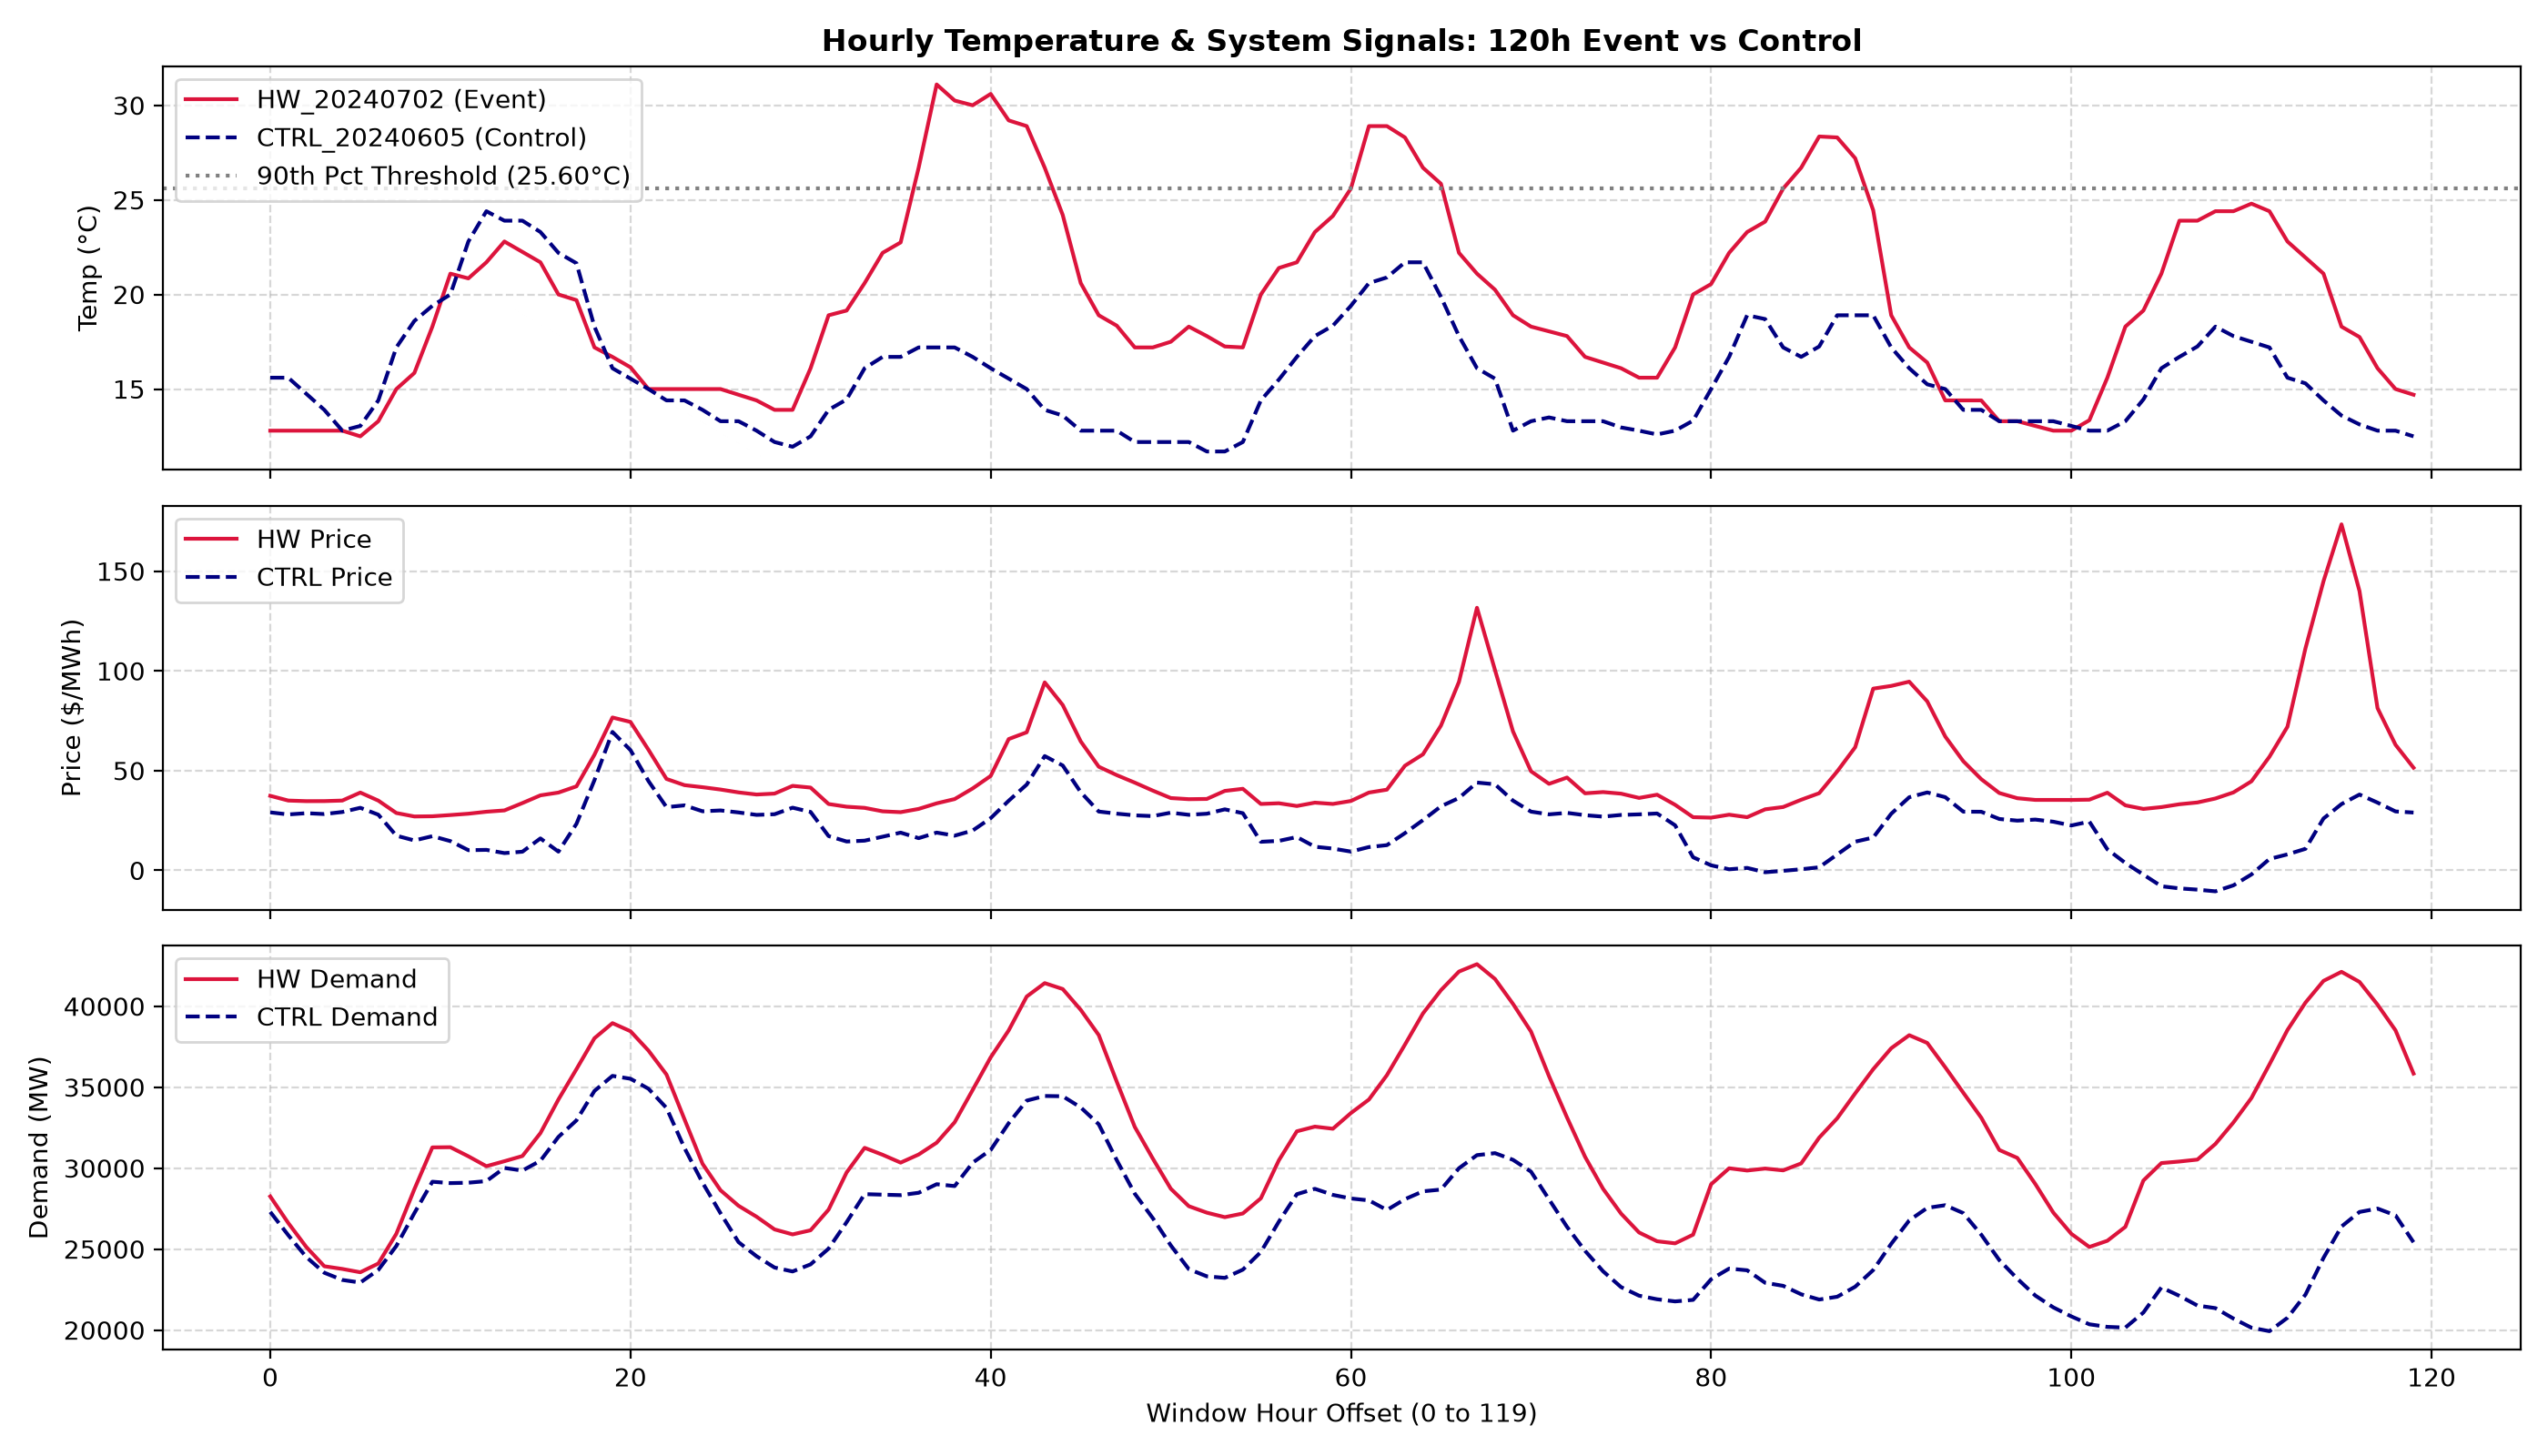
\includegraphics[width=0.88\textwidth]{figures/fig1_signals_time_series.png}
\caption{Illustrative 120-hour development pair: the July 2024 SFO heatwave and its June 2024 matched control. The figure shows aligned temperature, wholesale price, and demand; it demonstrates dataset structure and is excluded from confirmatory inference.}
\label{fig:signals}
\end{figure*}

\subsection{Catalogue records and scenario artifacts}

Each triplet index row records event, control, and blind IDs; UTC bounds; duration and row count; matching covariates; selection seed and version; eligibility; data-quality status; and gate outcome. Its Parquet bundle adds hourly phase labels and canonical signals. The multi-station catalogue adds station metadata, threshold and sample size, duration, temperature summaries, cumulative exceedance, onset/recovery, episode, eligibility, provisional state, exclusion reason, and source reference. Episodes are connected components after 24-hour expansion of each event interval; this reduces double-counting, although transitive chaining can form long components.

\begin{table*}[t]
\caption{Verified catalogue and benchmark characterization. Counts refer to different data objects and are not interchangeable.}
\label{tab:catalogue}
\small
\begin{tabular}{@{}p{0.24\textwidth}p{0.20\textwidth}p{0.40\textwidth}@{}}
\toprule
\textbf{Artifact} & \textbf{Verified size/coverage} & \textbf{Meaning} \\
\midrule
Original SFO event catalogue & 4 events, 2022--2024 within 2022--2025 screening & 1 development event and 3 confirmatory events \\
Frozen scenario index & 4 triplets; 12 windows; 120 rows per window & Event, matched control, and selected event-blind window per triplet \\
Confirmatory independent units & 3 historical triplets & Unit for H1--H5 classification; simulation cells are not events \\
Multi-station event catalogue & 25 station events, June--September 2022--2026 & 12 eligible, 9 excluded, 4 provisional; five primary stations \\
Regional episode catalogue & 15 episodes at 24-h connection buffer & 7 eligible, 5 excluded, 3 provisional; six usable paired episodes in the narrow retrospective static analysis \\
Extension benchmark windows & 12 controls and 240 selected ordinary windows & 20 ordinary windows per matrix event; overlap audit required \\
\bottomrule
\end{tabular}
\end{table*}

\section{Dataset Characterization, Quality, and Reproducibility}\label{sec:quality}

The extension screens June--September seasons, requiring at least 98\% valid daily maxima. SFO 2025 is excluded because only 119/122 days (97.54\%) are valid; the predeclared Sacramento fallback is not activated. Station-specific $P_{90}$ thresholds range from $25.6^{\circ}$C at SFO to $41.7^{\circ}$C at RDD, preventing a single coastal threshold from defining inland heat. Weather-only detection yields 25 station events and 15 episodes. All nine 2022 events pass weather eligibility and remain catalogue-visible, but the code excludes the entire year from joint evaluation because one EIA interval, 2022-06-13 17:00 UTC, is missing from the annual source gate. That timestamp lies outside every affected full event window. This is a conservative joint-source pipeline rule, not meteorological invalidity or evidence of missing data within those windows. A future event-window coverage gate could retain complete events; none is restored here. Four 2026 events are provisional pending calendar certification.

CSV artifacts expose catalogue, coverage, scenario, overlap, missingness, equal-service, and claim-decision records; JSON/JSONL manifests capture hashes, configurations, counts, source inventories, and git provenance; Parquet retains typed hourly and run-level data. Stable IDs link events, episodes, scenarios, matrix cells, and results. The matrix has 6,480 unique run IDs: 6,336 deployable and 144 oracle-reference cells.

\subsection{Record semantics and reuse}

Table~\ref{tab:schema} summarizes verified columns from public and locally generated machine-readable artifacts. Grains are joined by identifiers rather than approximate dates: \texttt{event\_id} links extension hourly signals and scenarios, \texttt{regional\_episode\_id} links spatially related events, and \texttt{run\_id} identifies one scenario--policy--facility--curve--load--seed cell. Researchers should preserve the stated simple or composite keys; hourly rows, windows, station events, episodes, and simulation runs are not interchangeable samples.

\begin{table*}[t]
\caption{Dataset schema: record grain, stable keys, representative fields, and quality controls.}
\label{tab:schema}
\small
\begin{tabular}{@{}p{0.14\textwidth}p{0.24\textwidth}p{0.34\textwidth}p{0.18\textwidth}@{}}
\toprule
\textbf{Record} & \textbf{Key/time} & \textbf{Representative fields} & \textbf{QC/links} \\
\midrule
Original hourly & Composite: \path{triplet_id}, \path{window_type}, \path{timestamp_utc} & \path{temperature_c}, \path{price_usd_per_mwh}, \path{carbon_g_per_kwh}, \path{demand_mw}, \path{phase_label} & 1,440 public rows; no observed nulls \\
Extension hourly & Composite: \path{event_id}, \path{timestamp_utc} & \path{temperature_c}, \path{price_usd_per_mwh}, \path{carbon_g_per_kwh}, \path{demand_mwh}, \path{phase} & 4,320 local rows; source-specific missing flags \\
Station event & Unique \path{event_id}; local/UTC bounds & \path{threshold_temperature_c}, \path{duration_hours}, \path{peak_temperature_c} & 25 rows; weather/joint eligibility \\
Regional episode & Unique \path{regional_episode_id}; component bounds & \path{member_event_count}, \path{station_codes}, \path{event_ids} & 15 rows; eligibility summary \\
Scenarios & Unique \path{control_id} or \texttt{ordinary\_\allowbreak window\_id} & \path{matched_event_id}, \path{duration_hours}, \path{candidate_rank}, \path{matching_score} or \path{stratum} & 12 controls; 240 ordinary windows \\
Execution & Unique \path{run_id}; \path{window_id} link & \path{execution_status}, \path{failure_category}, \texttt{completed\_processing\_slots}, \texttt{total\_facility\_energy\_kwh} & 6,480 rows; failed outcomes may be null \\
\bottomrule
\end{tabular}
\end{table*}

The catalogue supports complete-event trajectory analysis, alternative outcome-blind controls, common-window scheduler tests, and coverage/dependence audits. Reuse should retain source flags and full boundaries, handle overlap, and aggregate at the event or episode level. Additional evidence is required for claims about facility failures, marginal emissions, retail costs, or global heat.

Completeness is field-specific: a valid weather season may contain a later window without price, carbon, or forecast coverage, and successful execution cannot repair a source defect. Separate weather eligibility, joint-source eligibility, execution, and equal-service fields let users retain a valid weather catalogue without inheriting invalid forecast-aware conclusions.

\subsection{Reconstruction path and present limits}

The implemented path validates cached or acquired sources, harmonizes hourly records, detects weather-only events, and freezes scenarios, workloads, and the matrix. From the repository root in an installed Python 3.11+ development environment, the verified command-line entry points are:
\par\smallskip
{\small\ttfamily\noindent
python scripts/p12\_b2\_acquire\_sources.py --repo-root .\\
python scripts/p12\_b2\_detect\_events.py
\par}
\smallskip
The first command needs provider inputs and may need network access or credentials. Scenario freezing is implemented by the internal Python function \path{run_phase4_pipeline(repo_root=".")} rather than a command-line interface; it requires the local processed sources and manifests. Core dependencies include pandas, PyArrow, and PyYAML. Acquisition logs, coverage tables, freeze manifests, hashes, and row counts establish lineage. Raw \texttt{data/raw} and \texttt{data/v2/raw} and processed \texttt{data/v2/processed} are Git-ignored; CAISO historical access varies, and redistribution is provider-dependent. Syntax and entry points were checked without reacquiring data or rerunning experiments. A clean-checkout source-to-result reconstruction is not demonstrated.

The confirmatory archive contains frozen specifications, benchmarks, model artifacts, 756 execution rows, analyses, and checksums. A zero-resume rerun reproduced all run IDs and 44 audited scientific columns; seven analysis CSVs and four figure/status artifacts were byte-identical, and 54/54 payloads verified. This establishes same-environment artifact reproducibility, not independent source reconstruction or dependency portability.

\section{Benchmark Evaluation Framework}\label{sec:framework}

\subsection{Thermal, workload, forecast, and policy models}

The facility response is a controlled sensitivity. For curve $c$ and ambient temperature $T_t$,
\begin{equation}
\operatorname{PUE}_{c}(T_t)=\min\!\left(PUE_{\max,c},1.20+s_c\max(0,T_t-22)\right),
\end{equation}
and
\begin{equation}
P_{\mathrm{facility},t}=P_{\mathrm{IT},t}\operatorname{PUE}(T_t),\qquad
C_{\mathrm{eff},t}=\min\!\left(500,\frac{600}{\operatorname{PUE}(T_t)}\right)\ \mathrm{kW}.
\end{equation}
The low curve uses $s=0.010$ and $PUE_{\max}=1.45$; the primary medium curve uses $s=0.020$ and $PUE_{\max}=1.70$. Figure~\ref{fig:thermal} visualizes the modeled coupling.

\begin{figure*}[t]
\centering
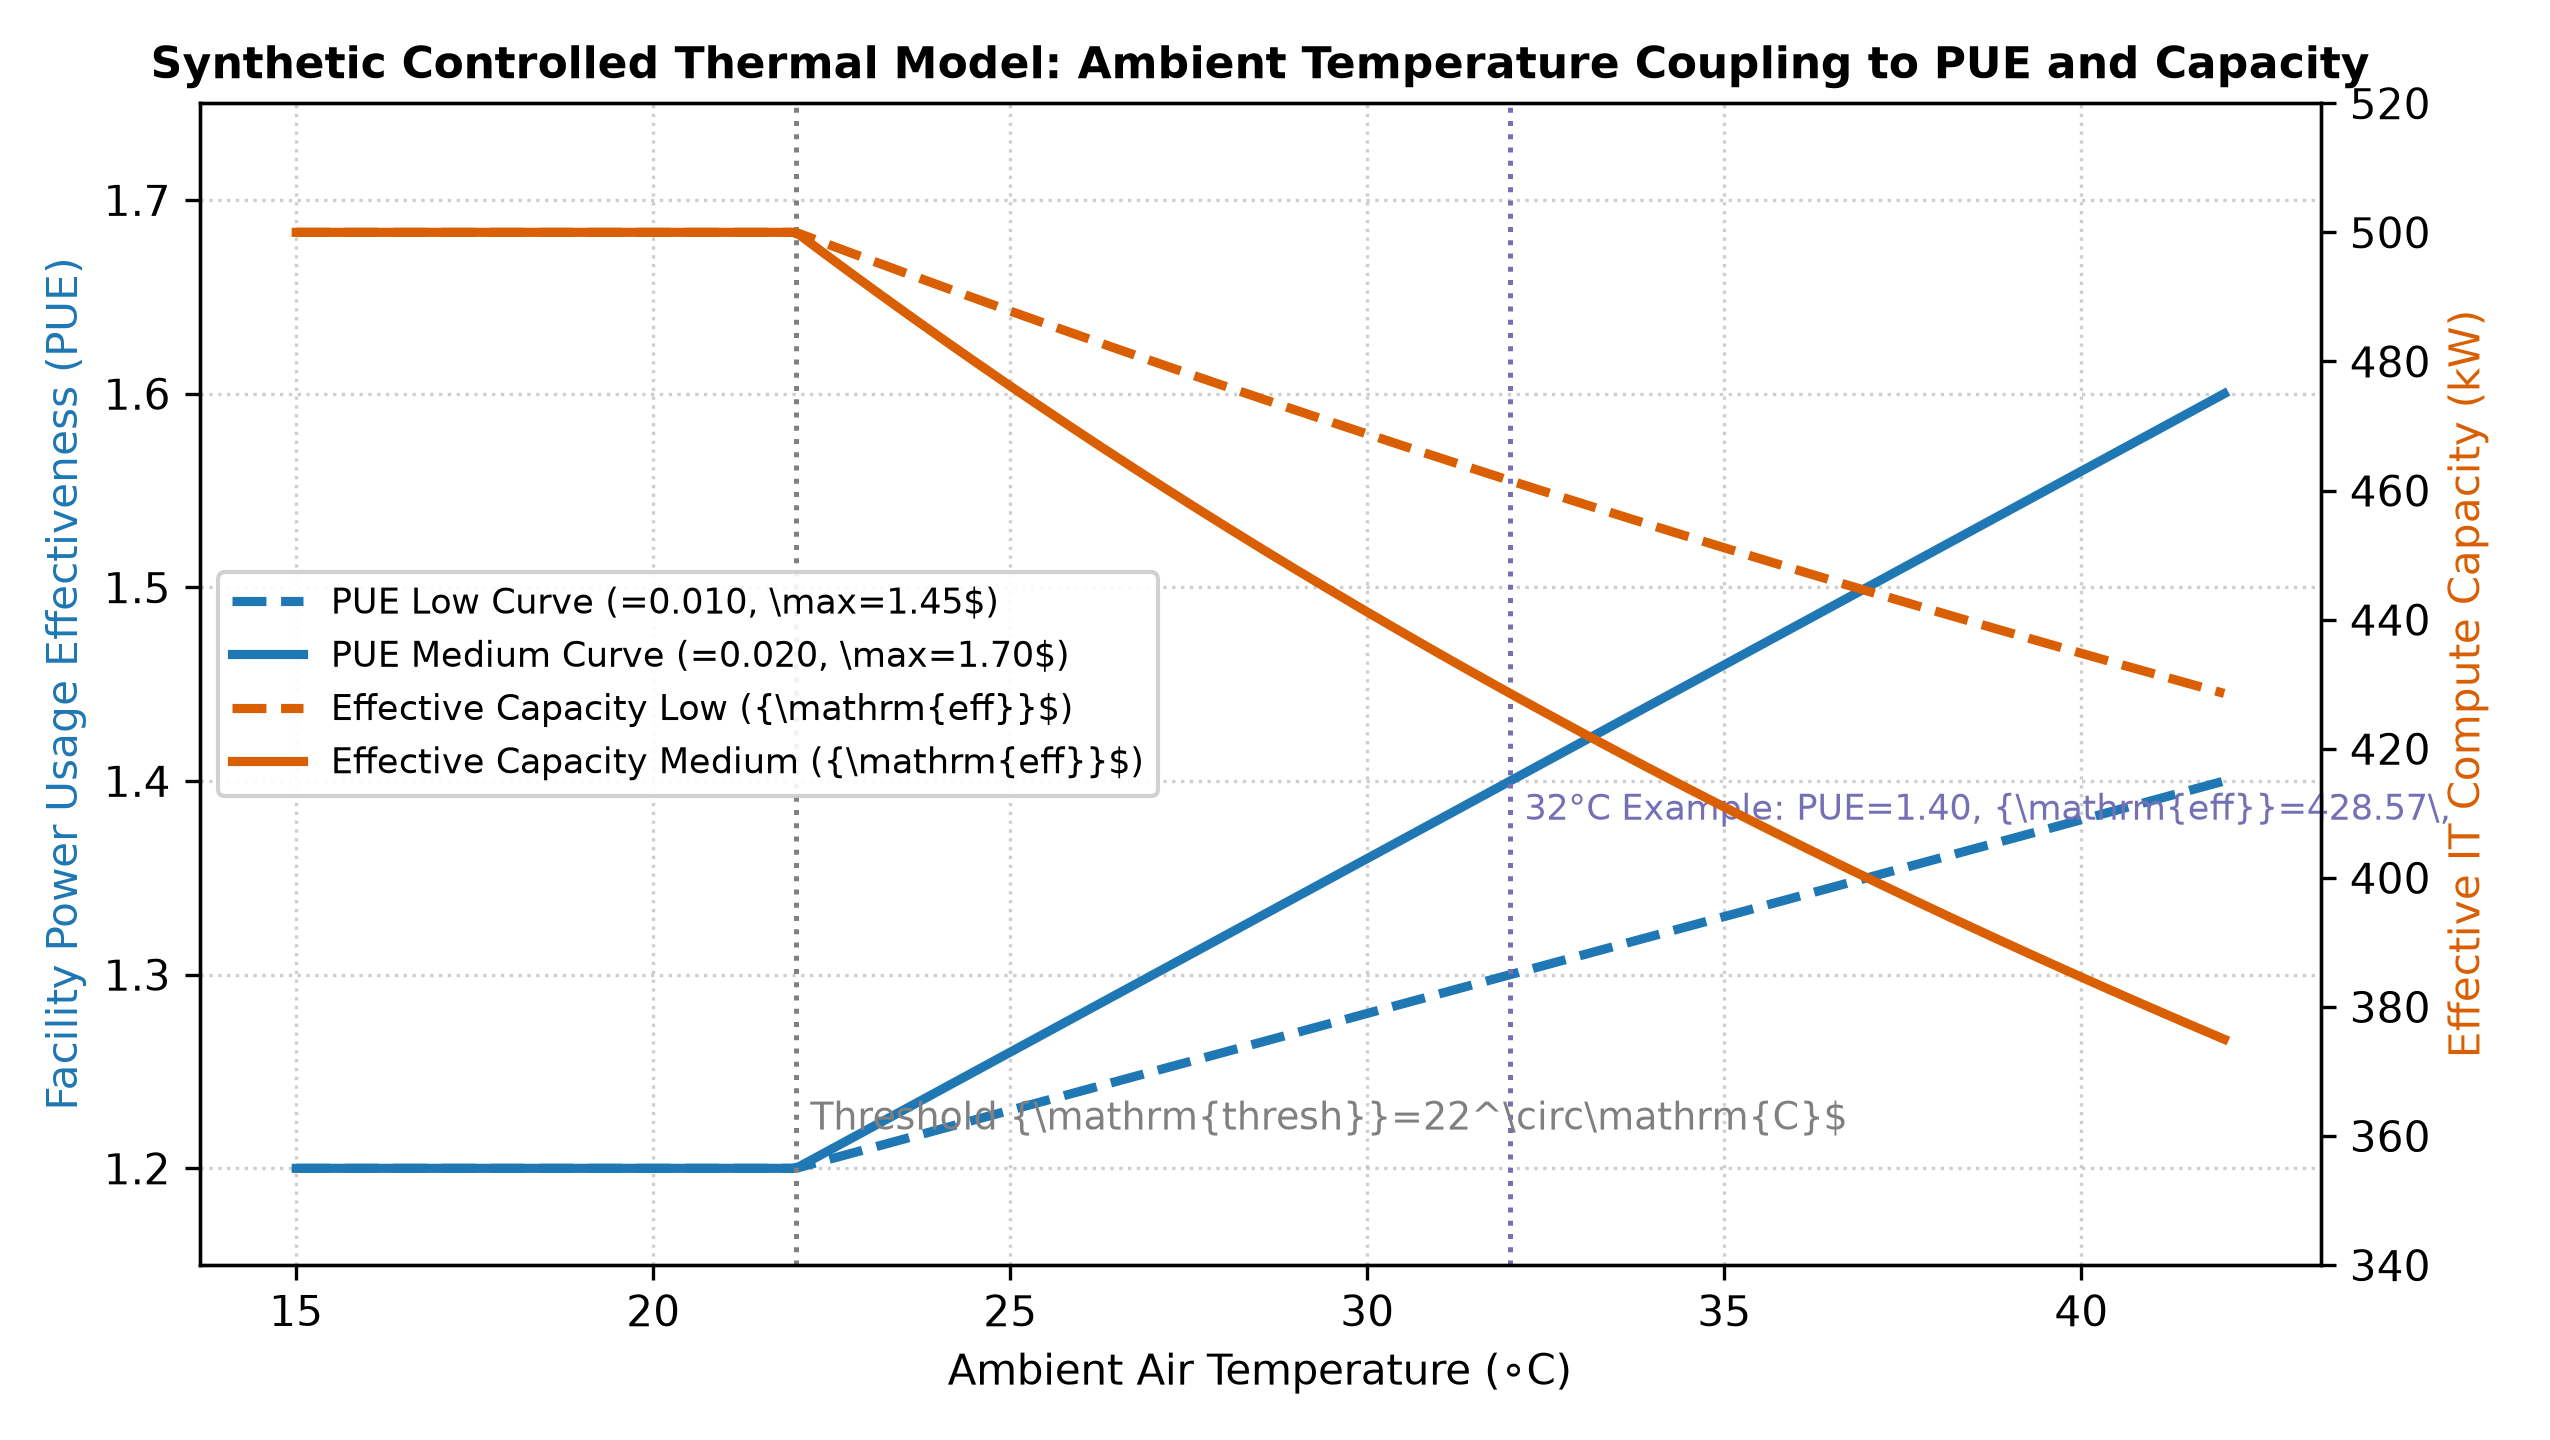
\includegraphics[width=0.77\textwidth]{figures/diag2_thermal_model.png}
\caption{Controlled temperature--PUE--capacity sensitivity. Above $22^{\circ}$C, modeled PUE rises and the 600~kW facility cap reduces usable IT power. These curves are synthetic sensitivities, not production-facility measurements.}
\label{fig:thermal}
\end{figure*}

Synthetic deadline-constrained jobs use seeds 20261016 and 20261017 at tested multipliers $\{1,2,3\}\times$. Common arrivals are preserved across policies. A 72-hour-input, 24-hour-output TinyTemperatureLSTM supplies the designated forecast; no forecast-source intervention is randomized. Six policy roles range from static scheduling through capacity/full-thermal awareness, calibrated and fixed HeatGuard margins, and a non-deployable hindsight oracle. The policies are evaluation subjects, not dataset contributions.

\begin{table*}[t]
\caption{Frozen benchmark matrix and policy roles.}
\label{tab:design}
\small
\begin{tabular}{@{}p{0.22\textwidth}p{0.49\textwidth}p{0.18\textwidth}@{}}
\toprule
\textbf{Policy/cohort} & \textbf{Information and coverage} & \textbf{Cells/status} \\
\midrule
Static, capacity, full thermal & Three deployable roles; event/control; 3 triplets, 2 facilities, 2 curves, 3 loads, 2 seeds, 2 objectives & 432 \\
Event-blind core & Same three policies and frozen factors in selected ordinary windows & 216 \\
HeatGuard calibrated/fixed & Power-capped, medium curve, carbon-first; event and control & 72; heuristic \\
Oracle full thermal & Realized future temperature; power-capped, medium, carbon-first & 36; non-deployable \\
\midrule
\textbf{Total} & 756 successful cells; independent units are the three historical triplets & 756 \\
\bottomrule
\end{tabular}
\end{table*}

\subsection{Metrics, equal service, and boundary aggregation}

Cost or carbon gaps are eligible only when both schedules complete the demanded service,
\begin{equation}
S_{\mathrm{demanded}}=S_{\mathrm{completed}}(A)=S_{\mathrm{completed}}(B).
\end{equation}
Of 540 seed-aggregated comparisons, 530 pass; all deployable comparisons pass, while ten exclusions involve the incomplete oracle. Outcomes include completion, violation hours, maximum exceedance, facility energy, cost, and production-average carbon proxy.

The tested feasibility boundary requires careful interpretation. For each workload seed, it is the largest feasible executed multiplier in $\{1,2,3\}\times$; the reported event boundary is the arithmetic mean of the two seed-specific maxima. Therefore, a reported 2.5$\times$ boundary means one seed was feasible through 2$\times$ and the other through 3$\times$. No 2.5$\times$ workload was executed, and the value is not a continuous capacity estimate.

\section{Experimental Results and Benchmark Utility}\label{sec:results}

The experiments test whether complete events expose thermal-feasibility limits or policy differences absent from selected ordinary windows. Table~\ref{tab:results} and Figure~\ref{fig:results} give the event-level record.

\begin{table*}[t]
\caption{Primary confirmatory findings as evidence of benchmark utility.}
\label{tab:results}
\small
\begin{tabular}{@{}p{0.07\textwidth}p{0.16\textwidth}p{0.49\textwidth}p{0.18\textwidth}@{}}
\toprule
\textbf{Test} & \textbf{Decision} & \textbf{Event-level evidence} & \textbf{Limit} \\
\midrule
H1 & Supported & Static seed-averaged boundary changes: $-0.5\times,-0.5\times,0\times$; median $-0.5\times$ & Coarse executed grid; $N=3$ \\
H2 & Partially supported & No boundary recovery; full-thermal violation reductions of 1.0 h and 0.5 h in applicable events & Capacity-aware gave no improvement \\
H3 & Partially supported & Event gaps 24/36, 24/36, 0/36; blind gaps 0/36; 48 tie-to-nontie transitions & Zero strict reversals; one control also 24/36 \\
H4 & Not estimable & No same-scheduler controlled forecast-source intervention & No causal forecast attribution \\
H5 & Not supported & Calibrated HeatGuard beat both comparators in 0/3 events & No superiority or coverage claim \\
\bottomrule
\end{tabular}
\end{table*}

\begin{figure*}[t]
\centering
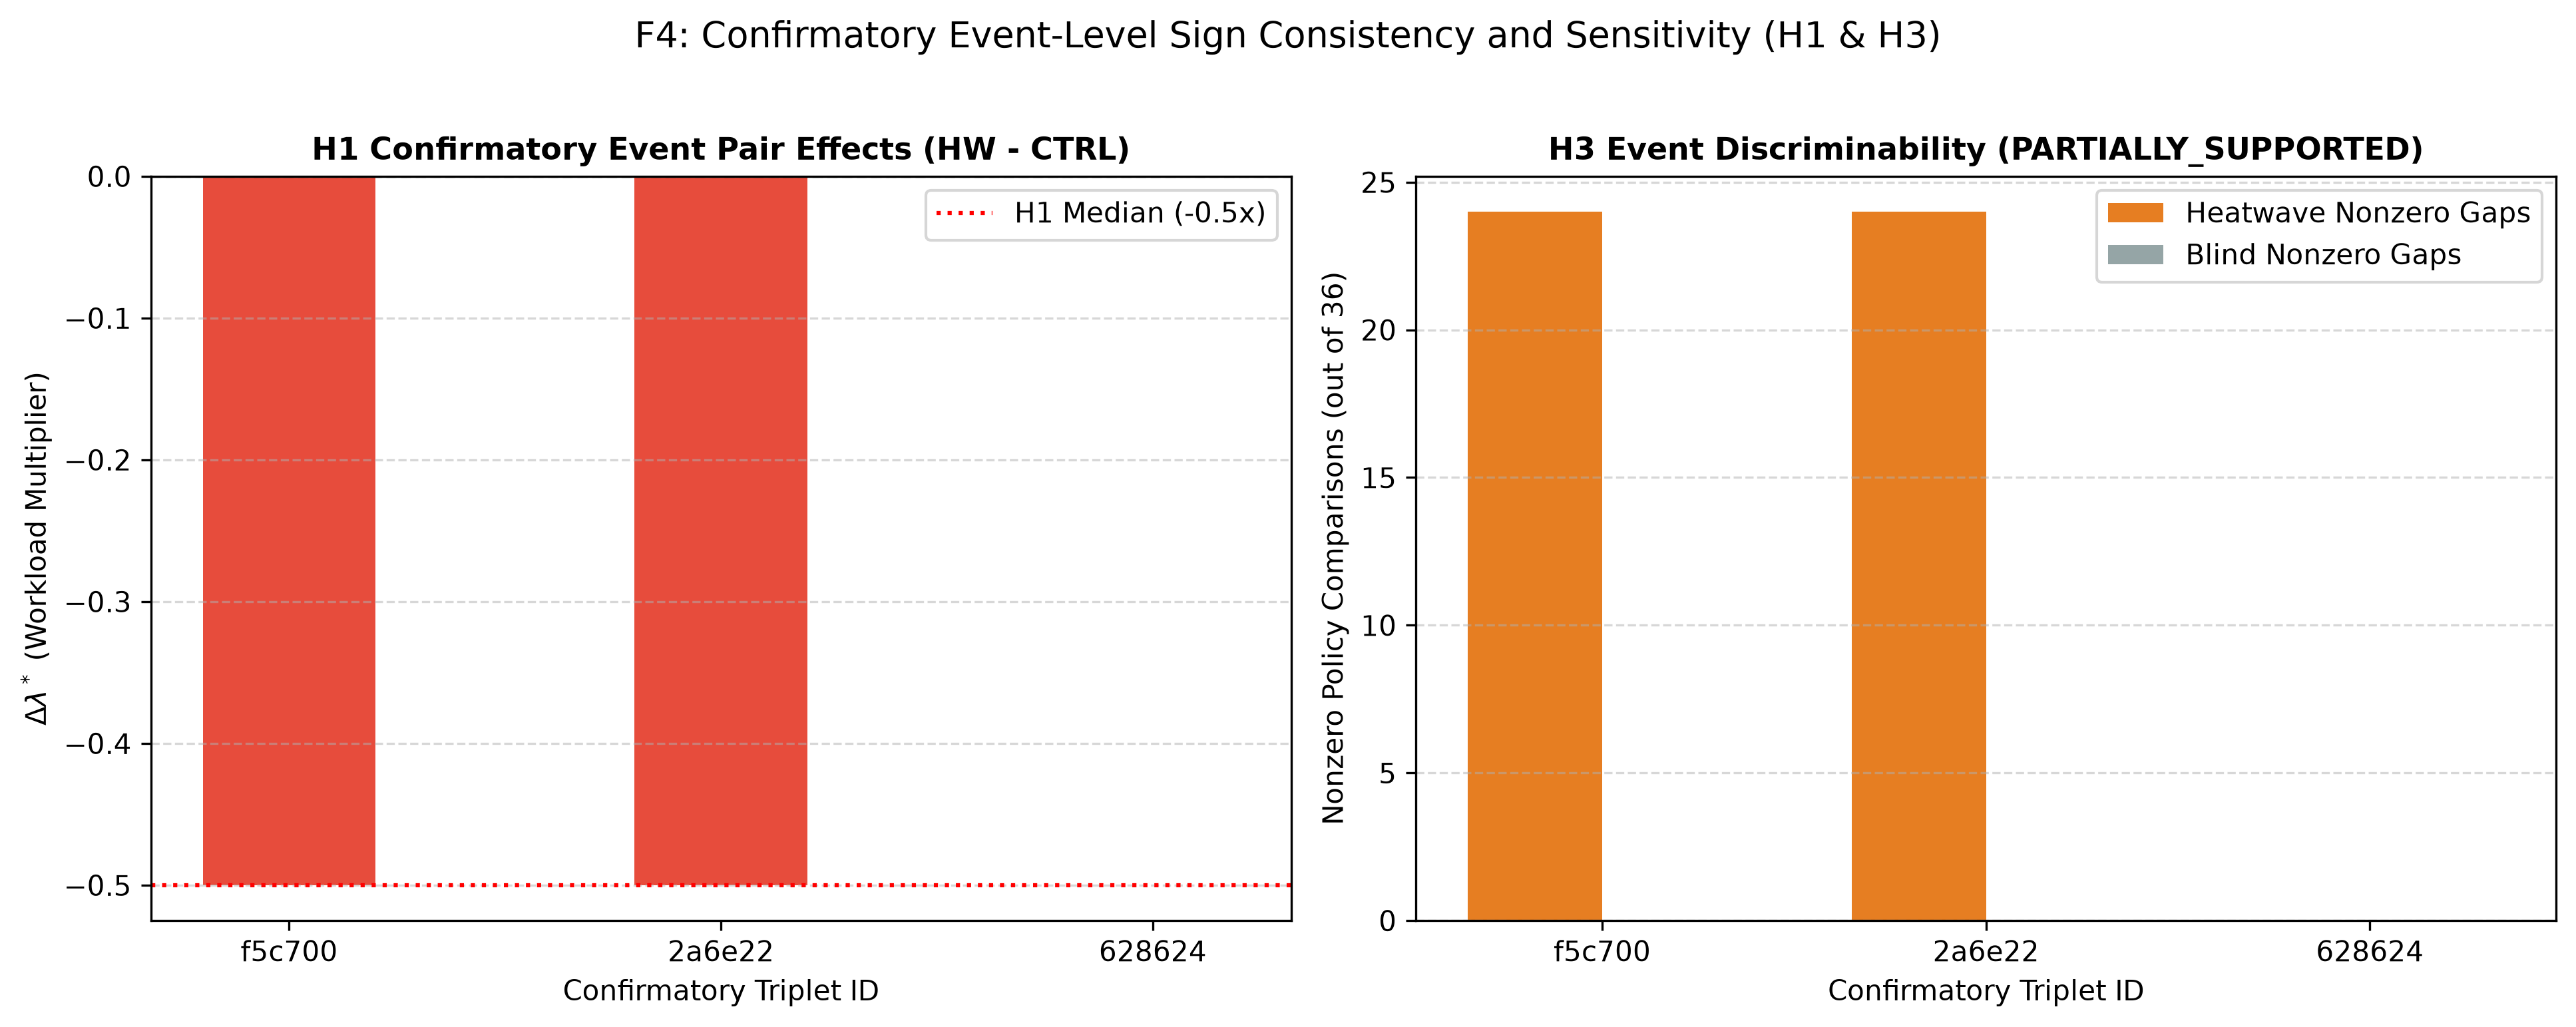
\includegraphics[width=0.76\textwidth]{figures/fig2_h1_sensitivity.png}
\caption{Primary results for three independent confirmatory events ($N=3$). The left panel shows seed-averaged feasibility-boundary differences; the right counts nonzero equal-service policy gaps. Two events separate where their selected blind windows do not, the third is null, and no comparison shows a strict policy-ranking reversal.}
\label{fig:results}
\end{figure*}

The first two complete events show a lower seed-averaged static feasibility boundary than their matched controls; the third is null. Preserving multi-day trajectories can expose modeled limits through the joint sequence of ambient temperature, capacity, deadlines, and grid signals, but this mechanism is not a causal explanation of the observed differences. Full thermal awareness reduces violation time without restoring a tested boundary; capacity awareness provides neither improvement.

The first two events separate policies where their selected event-blind windows do not, while the third does not separate them. No comparison strictly reverses policy order, and one matched control also separates policies, so the result is context sensitivity rather than heatwave-exclusive discrimination or a universal ranking. Equal-service filtering is essential: lower cost or carbon is interpretable only when both policies complete the same demanded work. Table~\ref{tab:results} retains the exact counts and classifications.

Forecast causality is not estimable because forecast source is never varied while holding the scheduler, workload, and scenario fixed; such an intervention is required to separate forecast information from policy behavior. Calibrated HeatGuard does not outperform both comparison policies in any event. These negative results prevent forecast accuracy and heuristic margins from being credited for effects the design cannot identify.

\section{California Multi-Station Dataset Extension and Quality Assessment}\label{sec:extension}

The five-station extension broadens catalogue coverage and supplies station metadata, station-specific thresholds, variable full-event windows, regional episodes, 12 matched controls, 240 selected ordinary windows, and a 6,480-cell experimental matrix. Of those cells, 5,448 succeeded and 1,032 failed: 936 for incomplete weather and 96 for missing forecasts. The curated event, episode, coverage, scenario, and missingness artifacts remain useful even though the forecast-aware conclusions failed scientific validation.

The validation audit found that the SFO model, scaler, and HeatGuard calibration were reused at four non-SFO stations despite a protocol prohibition; 3,960 unique non-SFO forecast-dependent run IDs are affected. Only 7/66 heatwave core-policy trios pass equal service, including 0/22 at both 2$\times$ and 3$\times$. Of 240 selected ordinary windows, 146 overlap another selected window, by up to 72 hours. Continuity analysis lacks hourly allocation/backlog state, and nine of ten planned robustness variants were not executed. Table~\ref{tab:audit} separates dataset value from invalid or incomplete conclusions.

\begin{table*}[t]
\caption{Validation audit of the California multi-station extension.}
\label{tab:audit}
\small
\begin{tabular}{@{}p{0.12\textwidth}p{0.38\textwidth}p{0.38\textwidth}@{}}
\toprule
\textbf{Item} & \textbf{Audit result} & \textbf{Interpretation} \\
\midrule
Catalogue & 25 events; 15 episodes & Exploratory; dependence flagged \\
Execution & 5,448 success; 1,032 failure & Failed cells unvalidated \\
Forecast & 3,960 run IDs affected & Forecast claims invalid \\
Service & 7/66 pass; 0/22 at high load & High-load savings invalid \\
Windows & 146/240 overlap; maximum 72 h & Dependent sample \\
Static & Six pairs; median +8.08 h & Retrospective result only \\
\bottomrule
\end{tabular}
\end{table*}

\section{Future Scope: A Global Heatwave Benchmark (2022--2026)}\label{sec:future}

After the end-semester examinations, a proposed 2022--2026 extension would select representative stations on multiple continents, document coverage and redistribution rights, apply region-specific weather-only thresholds and quality gates, and construct complete events, matched controls, and ordinary baselines before outcome inspection.

Harmonization would retain market structure, units, timestamps, price and carbon semantics, missingness, and flags. Episode and overlap graphs would support independent evaluation; forecasts would use station-appropriate training or preregistered fallbacks, with common workloads and equal service. Subject to source rights, the release would include manifests, licenses, immutable artifacts, schemas, dependency locks, clean-checkout instructions, and reproducibility records. No global dataset or experiment is claimed here.

\section{Conclusion}\label{sec:conclusion}

HeatTrace turns external weather and grid measurements into traceable event catalogues, complete-event scenarios, controls, ordinary windows, and quality records. Two of three confirmatory events expose a lower tested static boundary and policy gaps absent from selected ordinary windows; one event is null, no ordering reverses, and one control also separates policies. The multi-station extension expands the catalogue, not the validated scheduling claims. The evidence supports careful benchmark construction and bounded case-study utility, not global algorithmic or geographic conclusions.

\section*{Code and Data Availability}

Source code, frozen configurations, derived event and episode catalogues, scenario tables, manifests, workload traces, canonical result archives, and reproduction utilities are publicly available at \url{https://github.com/Sid-DudeD017/HeatTrace}; anonymous HTTP access was verified on 2026-11-20. The public tree includes the original hourly benchmark bundle and multi-station event, episode, scenario, matrix, result, and audit artifacts, but not the manuscript tree or the locally generated full multi-station hourly signal export. Raw and processed NOAA, CAISO, and EIA inputs are excluded by repository policy and must be obtained from the providers subject to their access and redistribution terms. The archive demonstrates same-environment result reproduction, not an independent clean-checkout source-to-result reconstruction.

\section*{Declarations}
\noindent\textbf{Funding}: [AUTHOR TO CONFIRM]. \textbf{Conflict of interest}: [AUTHOR TO CONFIRM].

\clearpage
\bibliography{references}

\end{document}
